 \documentclass[a4paper, 12pt]{article}
\usepackage{amssymb,amsfonts,amsmath}
\usepackage{bm}

\usepackage{graphicx}

\addtolength{\oddsidemargin}{-.875in}
\addtolength{\evensidemargin}{-.875in}
\addtolength{\textwidth}{1.75in}
\addtolength{\topmargin}{-.875in}
\addtolength{\textheight}{1.75in}

\usepackage{ascmac} % textbox

%\usepackage[normalem]{ulem}

\setlength{\parindent}{0pt}
\setlength{\parskip}{0.5em}

\begin{document}
% \pagestyle{plain}

\begin{center}
\begin{Large}
Dynamic programming
\end{Large}\\
\ \\
Naoki Masuda\\
Professor, Gilbert S.\,Omenn Department of Computational Medicine and Bioinformatics\\
Professor, Department of Mathematics\\
\ \\
UM Math Circle, 2/19/2026 
\end{center}

\section{Mouse in a maze and dynamic programming}

We can still do the maze problem by hand if the maze has 3 stages.\\
However, what if there are 4 stages? (Q: How many possible choices?)\\
How about 5 stages? (Q: how many possible choices?)

\bigskip

Let's introduce a new idea called ``\underline{backward induction}''.\\
It is an important component of ``\underline{dynamic programming}''.
\begin{itemize}
\item Not about coding.
\item But it is a key \underline{mathematical} technology used in ``reinforcement learning'' used in ``machine learning''.
\end{itemize}

\begin{center}
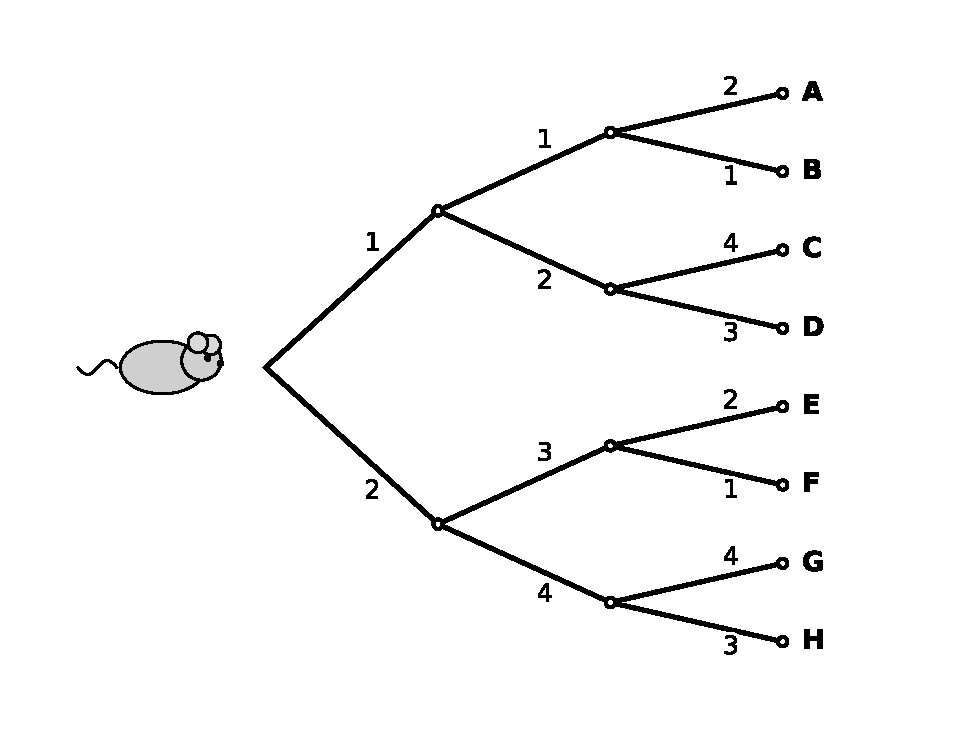
\includegraphics[width=0.8\textwidth]{dp_maze_tree_3stages_type0.pdf}
\end{center}

Let's name the internal nodes.

\begin{center}
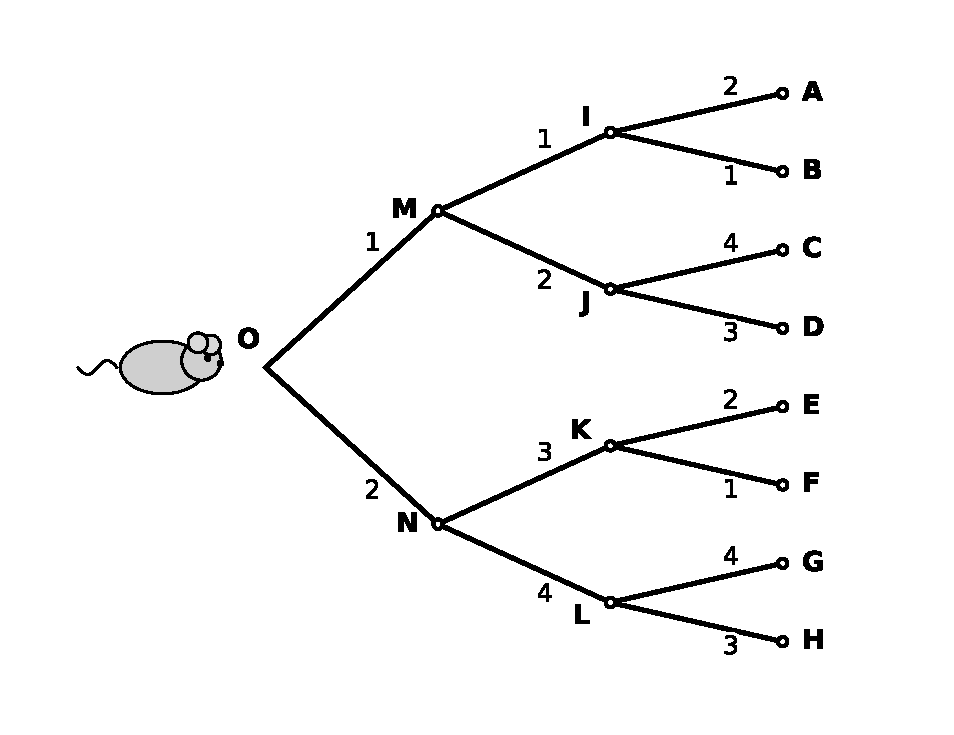
\includegraphics[width=0.8\textwidth]{dp_maze_tree_3stages_internal_nodes_labeled_type0.pdf}
\end{center}

\underline{Bellman equation}
\begin{equation*}
V(\text{M}) = \underbrace{\text{max over all choices}}_{\text{go to I or J}} \left\{ 1 + V(\text{I}), 2 + V(\text{J}) \right\} 
\end{equation*}

In this example, $V(\text{I}) = 2$ and $V(\text{J}) = 4$, so

\begin{itemize}
\item What's $V(\text{M})$?
% $\to$ $6$.\\
\item Which branch should the mouse select at location M?
\item What's $V(\text{N})$ and $V(\text{O})$?
\item Based on this, what's the best path starting location O?
\end{itemize}

The Bellman equation is used in 
\begin{itemize}
\item robots, cars, finding best routes
\item delivery companies (UPS, Fedex) to find fastest and cheapest ways
\item banks findindg the best way to invest money over time
\item hospital scheduling staff
\item $\cdots$
\end{itemize}

How to do this?
\begin{itemize}
\item Work backward.
\item Determine the \underline{value} of each \underline{state} ($=$ location)
\end{itemize}

\begin{description}

\item[Problem 1] In the following maze, get the mouse's optimal path and the total reward the mouse gets by taking the optimal path. Use backward induction.

\begin{center}
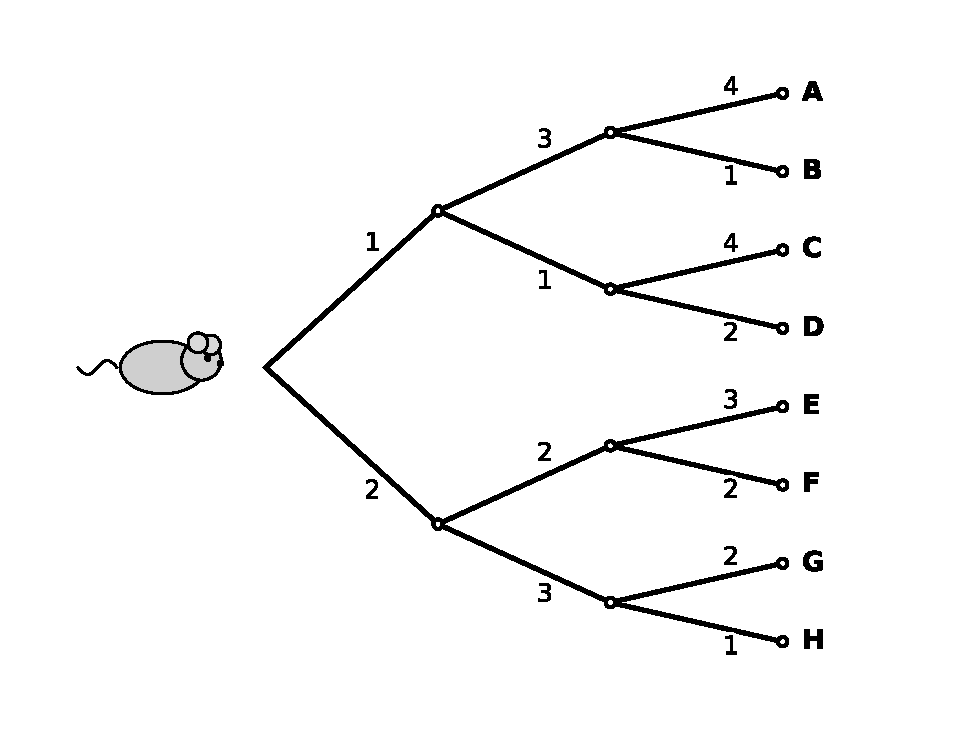
\includegraphics[width=0.8\textwidth]{dp_maze_tree_3stages_type1.pdf}
\end{center}


\newpage
\clearpage

\item[Problem 2] How about the following maze? Get the optimal path and total reward.

\begin{center}
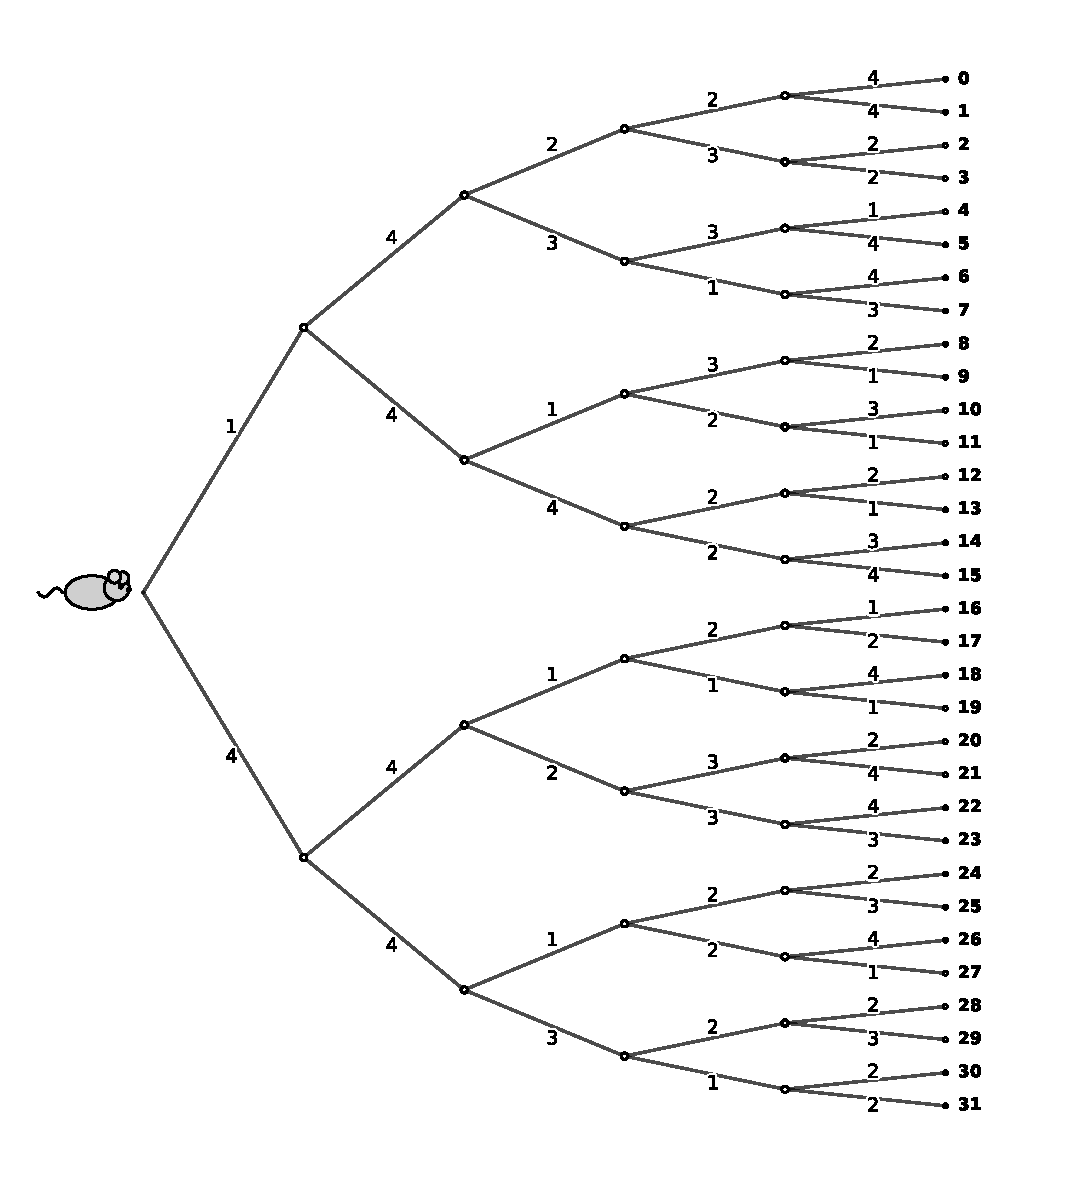
\includegraphics[width=\textwidth]{dp_maze_tree_5stages.pdf}
\end{center}

\newpage
\clearpage

\item[Problem 3] How about this uneven tree? Get the optimal path and total reward.
A long path is not necessarily better. 

\noindent
Now the rewards are placed on nodes rather than branches, but it does not matter. Mice do not care!

\noindent
Start by setting $V(A) = 7$, $V(B) = 1$, $V(C) = 2$, and so forth. As usual, work backward (from right to left of the figure).

\begin{center}
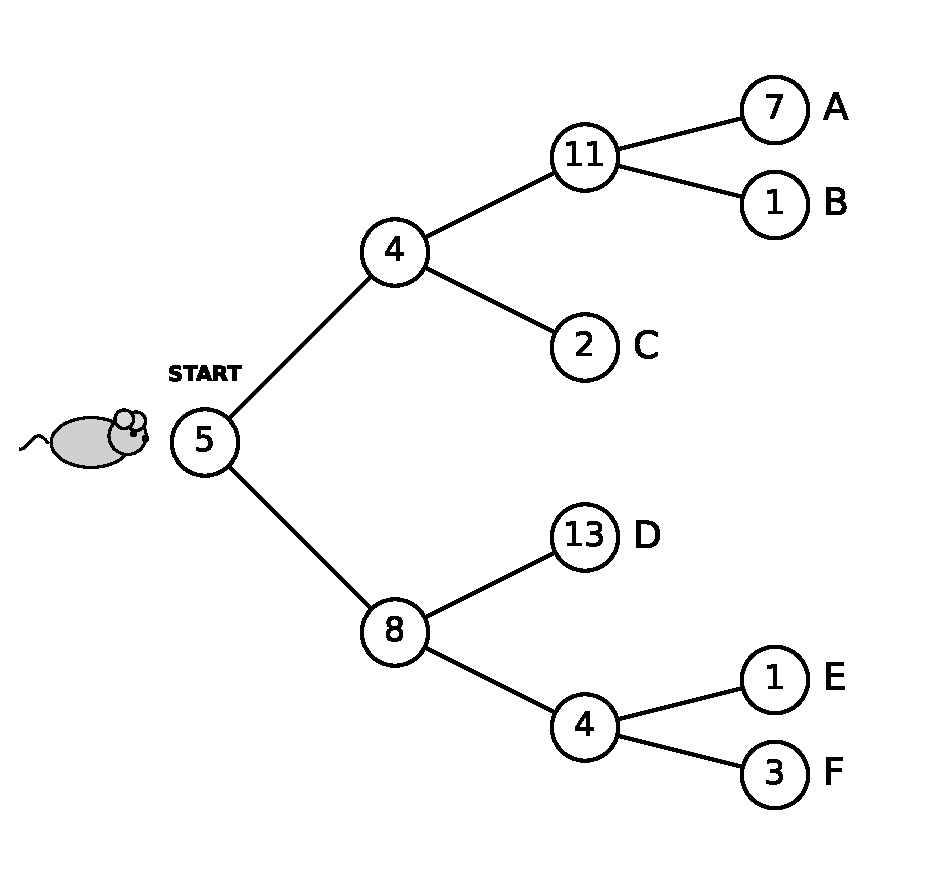
\includegraphics[width=0.9\textwidth]{dp_maze_tree_incomplete.pdf}
\end{center}

\newpage
\clearpage

\item[Problem 4] How about the following square maze? The mouse is only allowed to go RIGHT or DOWN.

\begin{center}
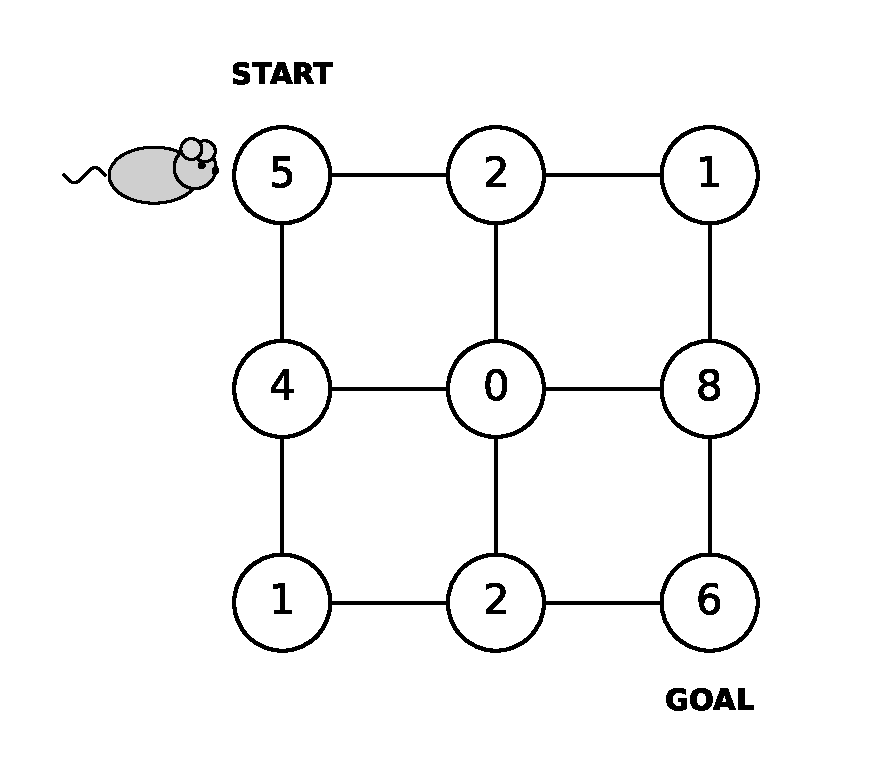
\includegraphics[width=0.6\textwidth]{dp_maze_square_3by3.pdf}
\end{center}

\newpage
\clearpage

\item[Problem 5] How about the following bigger square maze? The mouse can only go RIGHT or DOWN.

\begin{center}
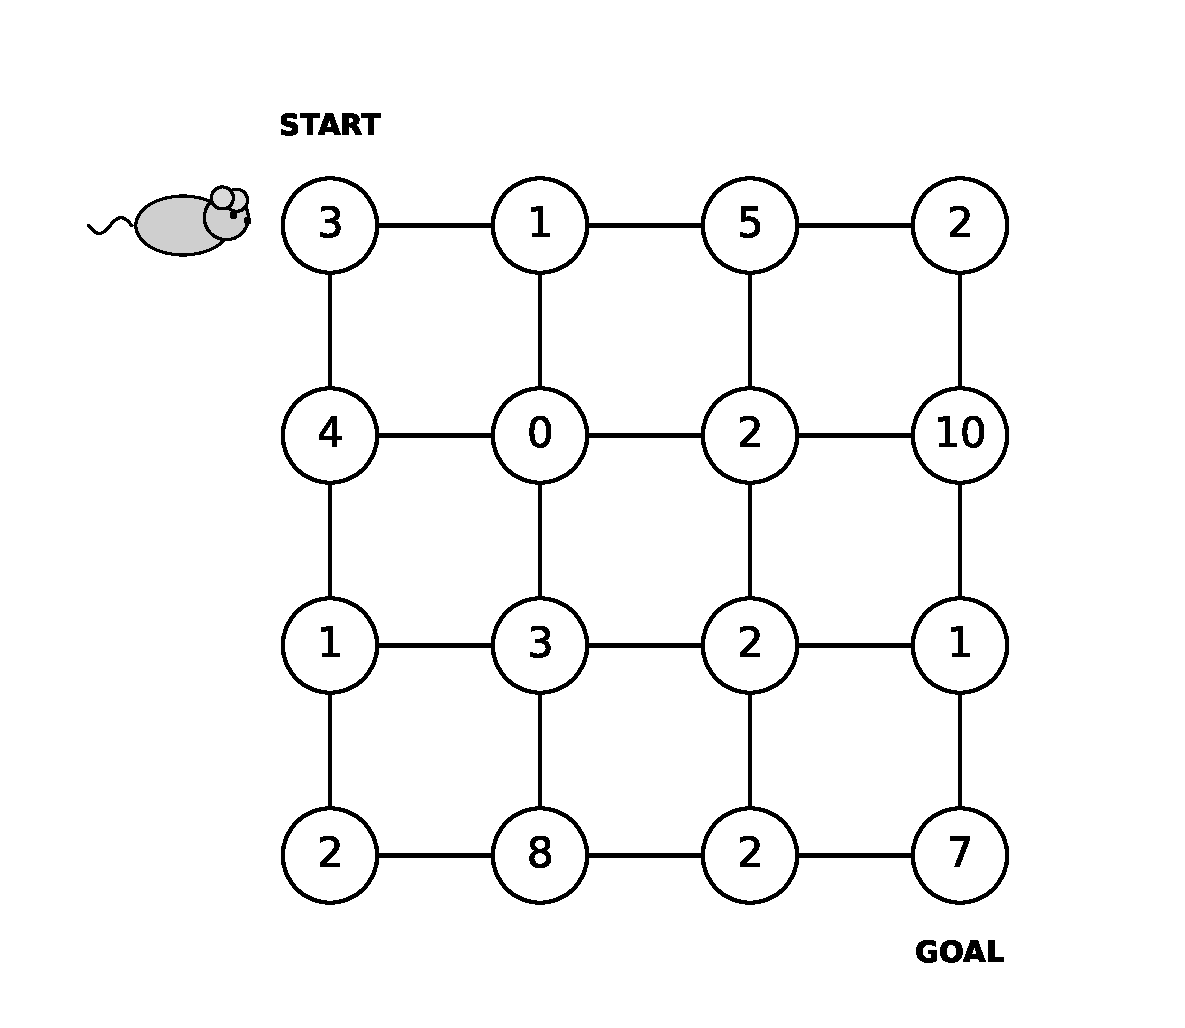
\includegraphics[width=0.8\textwidth]{dp_maze_square_4by4.pdf}
\end{center}

\end{description}

\newpage
\clearpage

\section{Jumpy frog path problem}

There are stepping stones in a river, and there is a frog.

\begin{center}
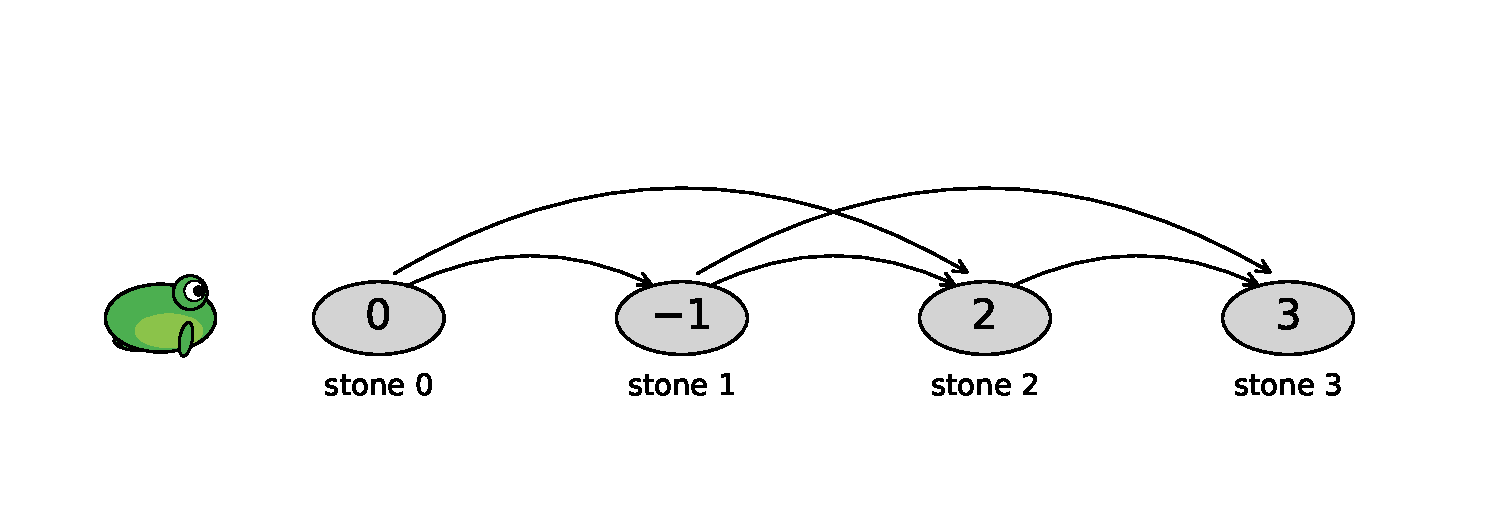
\includegraphics[width=0.8\textwidth]{frog_stones_1.pdf}
\end{center}

A frog is on stone 0 and wants to go to stone 3. In each jump, the frog can either go to the next stone or skip one stone. On each stone, there is a reward (negative value meaning punishment) the frog can get (food, poison, predation risk, etc.). What's the best path the frog should take?

Let's do this one together:

\bigskip

Q: How many possible paths? 

\begin{enumerate}

\item Write the Bellman equation:

\begin{equation*}
V(k) = (\text{reward at stone } k) + \max \left\{ V(k+1), V(k+2) \right\}.
\end{equation*}

\item Figure out what we know initially:

Base case: $V(3) = \text{reward at stone } 3 = 3$.

\item Do ``backward induction'' using the Bellman equation:

\begin{equation*}
V(2) = (\text{reward at stone 2}) + V(3) = 2 + 3 = 5.
\end{equation*}
(Note that the frog does not have a choice at stone 2.)

\begin{align*}
V(1) &= (\text{reward at stone 1}) + \max \left\{ V(2), V(3) \right\} = -1 + \max \left\{ 5, 3 \right\} = 4,\\
V(0) &= (\text{reward at stone 0}) + \max \left\{ V(1), V(2) \right\} = 0 + \max \left\{ 4, 5 \right\} = 5.
\end{align*}

\item Say the solution:

The optimal path is $0 \to 2 \to 3$.\\
The total reward the frog gets is $V(0)$, which is $5$.

\end{enumerate}

\newpage
\clearpage

\begin{description}

\item[Problem 6] How about the following step stone sequence? Optimal path and total reward?

The Bellman equation for this game is:
%
\begin{equation*}
V(k) = \begin{cases}
R(k) + \max \left\{ V(k+1), V(k+2) \right\} & \text{if } k= 0, \ldots, 4 \ (\text{the frog has two choices}),\\
R(k) + \max \left\{ V(k+1) \right\} & \text{if } k= 5, 6 \ (\text{the frog has just one choice}).\\
\end{cases}
\end{equation*}
$R(k)$ means the reward received at stone $k$. 

\bigskip

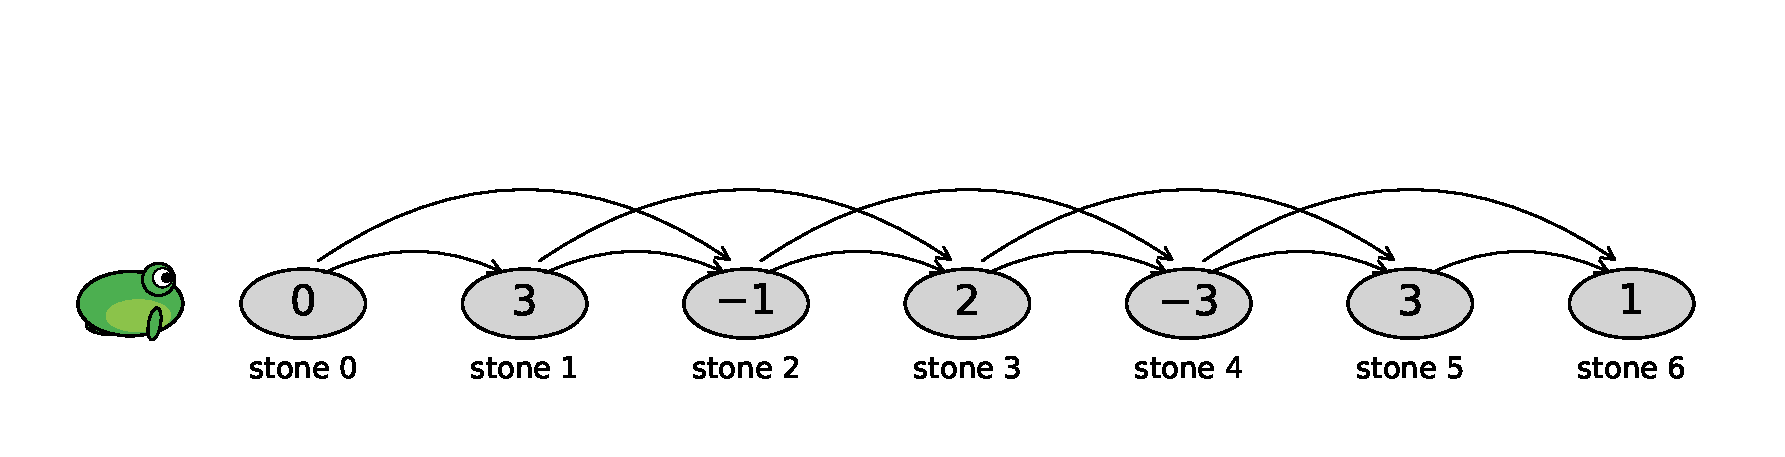
\includegraphics[width=0.9\textwidth]{frog_stones_2.pdf}

\newpage
\clearpage

\item[Problem7] How about the following case? The frog can now go to the next stone, skip two stones, or skip four stones.

Now the Bellman equation is
%
\begin{equation*}
V(k) = \begin{cases}
R(k) + \max \left\{ V(k+1), V(k+3), V(k+5) \right\} & \text{if } k= 0, \ldots, 7 \ (\text{the frog has three choices}),\\
R(k) + \max \left\{ V(k+1), V(k+3) \right\} & \text{if } k= 8, 9 \ (\text{the frog has two choices}),\\
R(k) + \max \left\{ V(k+1) \right\} & \text{if } k= 10, 11, 12 \ (\text{the frog has just one choice}).\\
\end{cases}
\end{equation*}

\bigskip

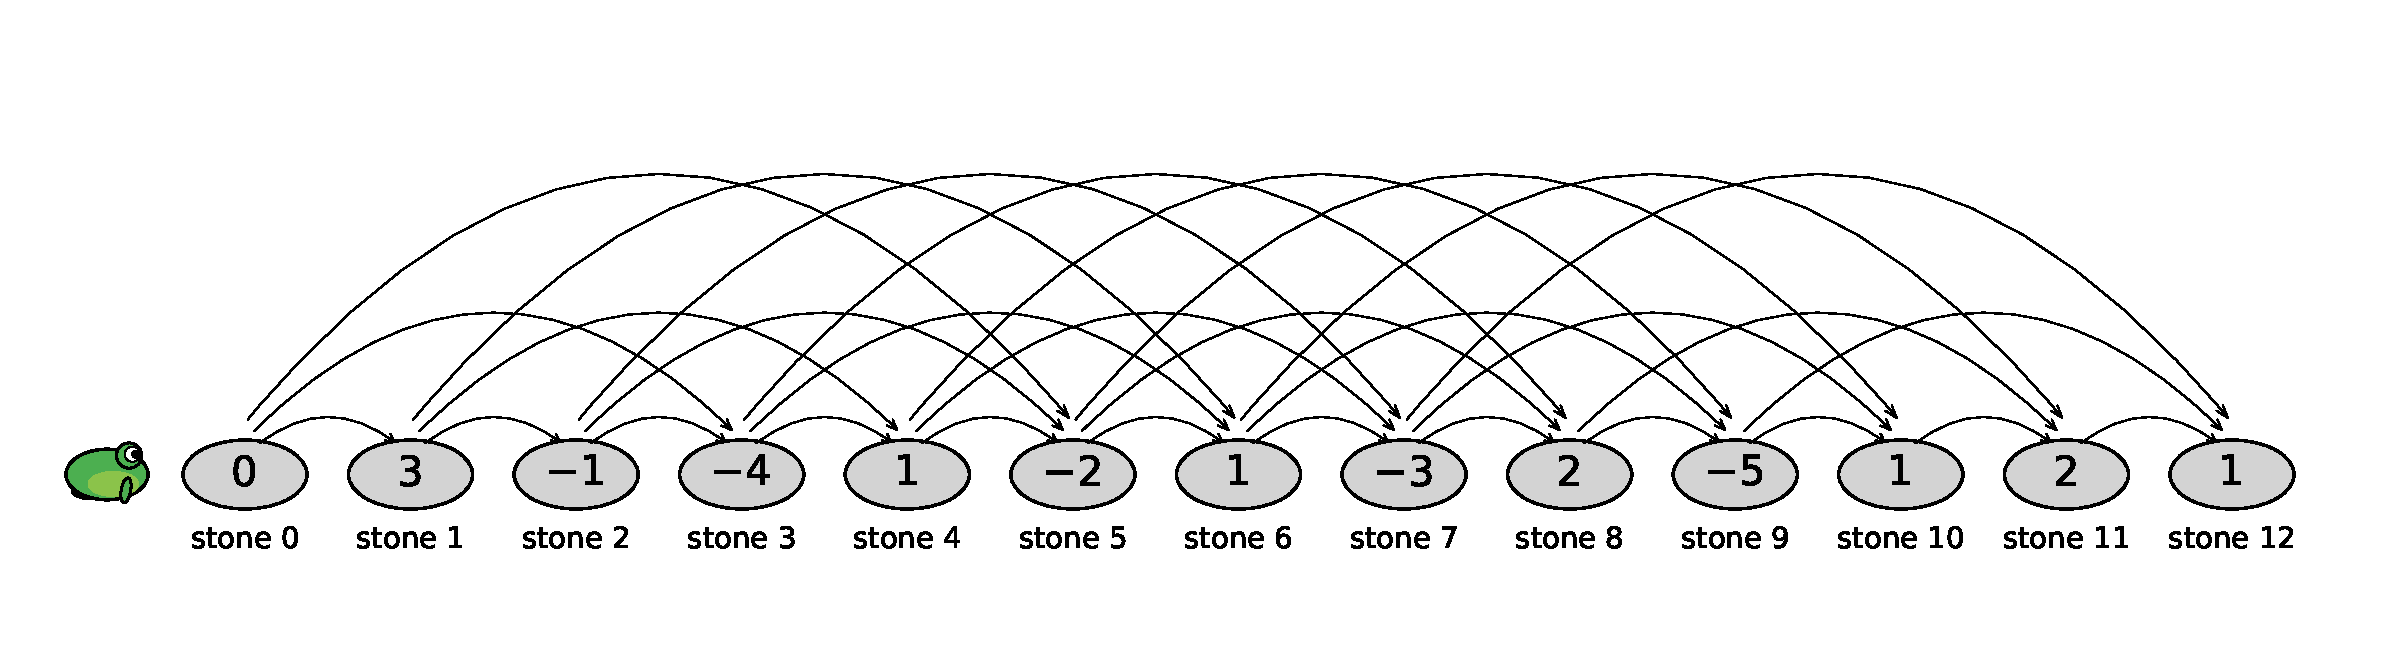
\includegraphics[width=\textwidth]{frog_stones_3.pdf}

\end{description}

\newpage
\clearpage

\section{Discounted candy collection}

You are in room 0.

\begin{center}
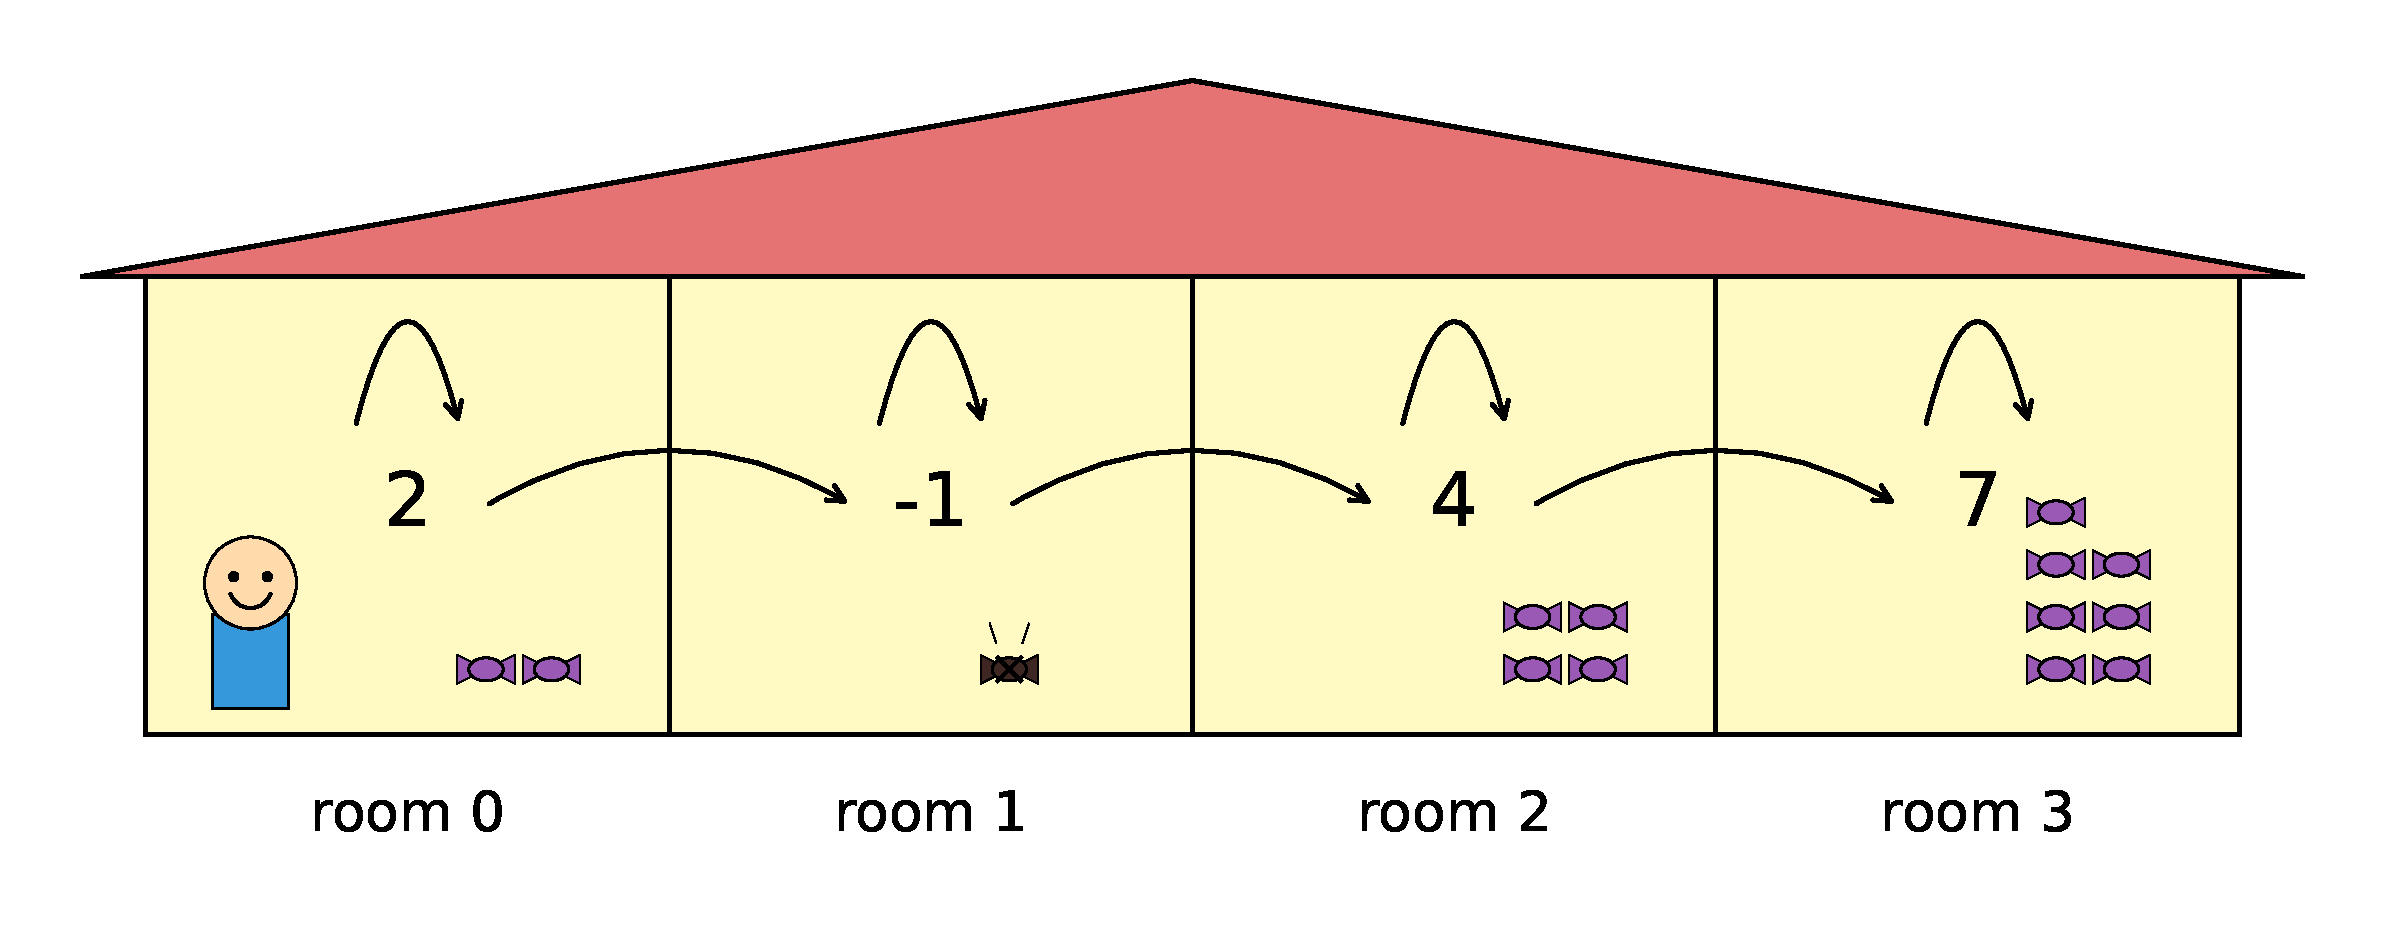
\includegraphics[width=0.8\textwidth]{candy_collection_1.pdf}
\end{center}

\begin{itemize}
\item You can either move RIGHT (to the next room) or STAY each day.
\item Each room has a candy dispenser of a different reward.
\item It may dispense a bitter candy! (See room 1).
\item It dispenses the known number of candies ($2$, $-1$, $4$, or $7$ depending on the room) each day.
\end{itemize}

Q: What would you do?

\bigskip

However, for me, what I get now is more important than what I get in the future.
\begin{itemize}
\item This is called ``discounted utility''. Appearing in economics theory, experimental psychology, etc.
\end{itemize}

So, what you want to maximize is:
\begin{equation}
\text{reward}(t) + \frac{1}{2} \text{reward}(t+1) + \frac{1}{4}\text{reward}(t+2) + \frac{1}{8}\text{reward}(t+3) + \cdots.
\end{equation}
$t$ is today, $t+1$ is tomorrow, $t+2$ is the day after tomorrow, etc.

You can reach room 3 in three days, but the seven candies you can get after 3 days give you a $\frac{1}{8}\times 7$ value only. Should you go there or stay in room 0?

\bigskip

Let's do this problem together.

\begin{enumerate}

\item{Write down the Bellman equation}

\begin{equation}
V(s) = R(s) + \max \left\{ \frac{1}{2}V(s), \frac{1}{2}V(s+1) \right\}.
\end{equation}
\begin{itemize}
\item $V(s)$ is the value of the room $s$.
\item The first option is STAY, and the second option is RIGHT.
\item $R(s)$ is the reward you get today in room $s$ (then you decide to STAY or go RIGHT).
\end{itemize}

\item Figure out what we know initially:

Nothing we can do. We do not know even $V(3)$ yet.

\item Do ``backward induction'' using the Bellman equation:

\begin{equation}
V(3) = R(3) = \frac{1}{2}V(3) = 7 + \frac{1}{2} V(3).
\end{equation}
(You can only STAY if you are in room 3.)\\

\bigskip

Q: $V(3)$?
%
% $\to$ A: $V(3) = 14$.

\bigskip

Today, you get 7, tomorrow's candy is counted as 3.5, the day after tomorrow's is 1.75, $\ldots$ $\to$ total is $14$.

\begin{equation*}
V(2) = 4 + \max \left\{ \frac{1}{2} V(2), \frac{1}{2} V(3) \right\}.
\end{equation*}
If STAY in room 2 is better, then $V(2) = 4 + \frac{1}{2} V(2)$, which leads to $V(2) = 8$.\\
If (going) RIGHT in room 2 is better, then $V(2) = 4 + \frac{1}{2} V(3) = 4 + \frac{1}{2} \times 14 = 11$.\\
So, better to go RIGHT if you are in room 2, and $V(2) = 11$.

\begin{equation*}
V(1) = -1 + \max \left\{ \frac{1}{2} V(1), \frac{1}{2} V(2) \right\}.
\end{equation*}
If STAY in room 1 is better, then $V(1) = -1 + \frac{1}{2} V(1)$, which leads to $V(1) = -2$. This sounds really bad.\\
If (going) RIGHT in room 1 is better, then $V(1) = -1 + \frac{1}{2} V(2) = \frac{9}{2}$.\\
So, better to go RIGHT if you are in room 1, and $V(1) = \frac{9}{2}$.

\begin{equation*}
V(0) = 2 + \max \left\{ \frac{1}{2} V(0), \frac{1}{2} V(1) \right\}.
\end{equation*}
If STAY in room 0 is better, then $V(0) = 2 + \frac{1}{2} V(0)$, which leads to $V(0) = 4$.\\
If (going) RIGHT in room 0 is better, then $V(0) = 2 + \frac{1}{2} V(1) = \frac{17}{4}$, which is larger than $4$.\\
So, better to go RIGHT if you are in room 0, and $V(0) = \frac{17}{4}$.

\item Say the solution:

The optimal behavior is go RIGHT RIGHT RIGHT toward room 3.

\end{enumerate}

\newpage

\begin{description}

\item[Problem 8] With a ``discount factor'' $r = \frac{1}{2}$, the best solution was to go RIGHT RIGHT RIGHT.\\
What if you \textit{really} want to the candy now than later?\\
Change the discount factor from $r = \frac{1}{2}$ to $r = \frac{1}{8}$, and get $V(3)$, $V(2)$, $V(1)$, and $V(0)$ to figure out the optimal behavior.\\

\newpage

\item[Problem 9] What is the optimal behavior in the following case with $r = \frac{1}{2}$?

\begin{center}
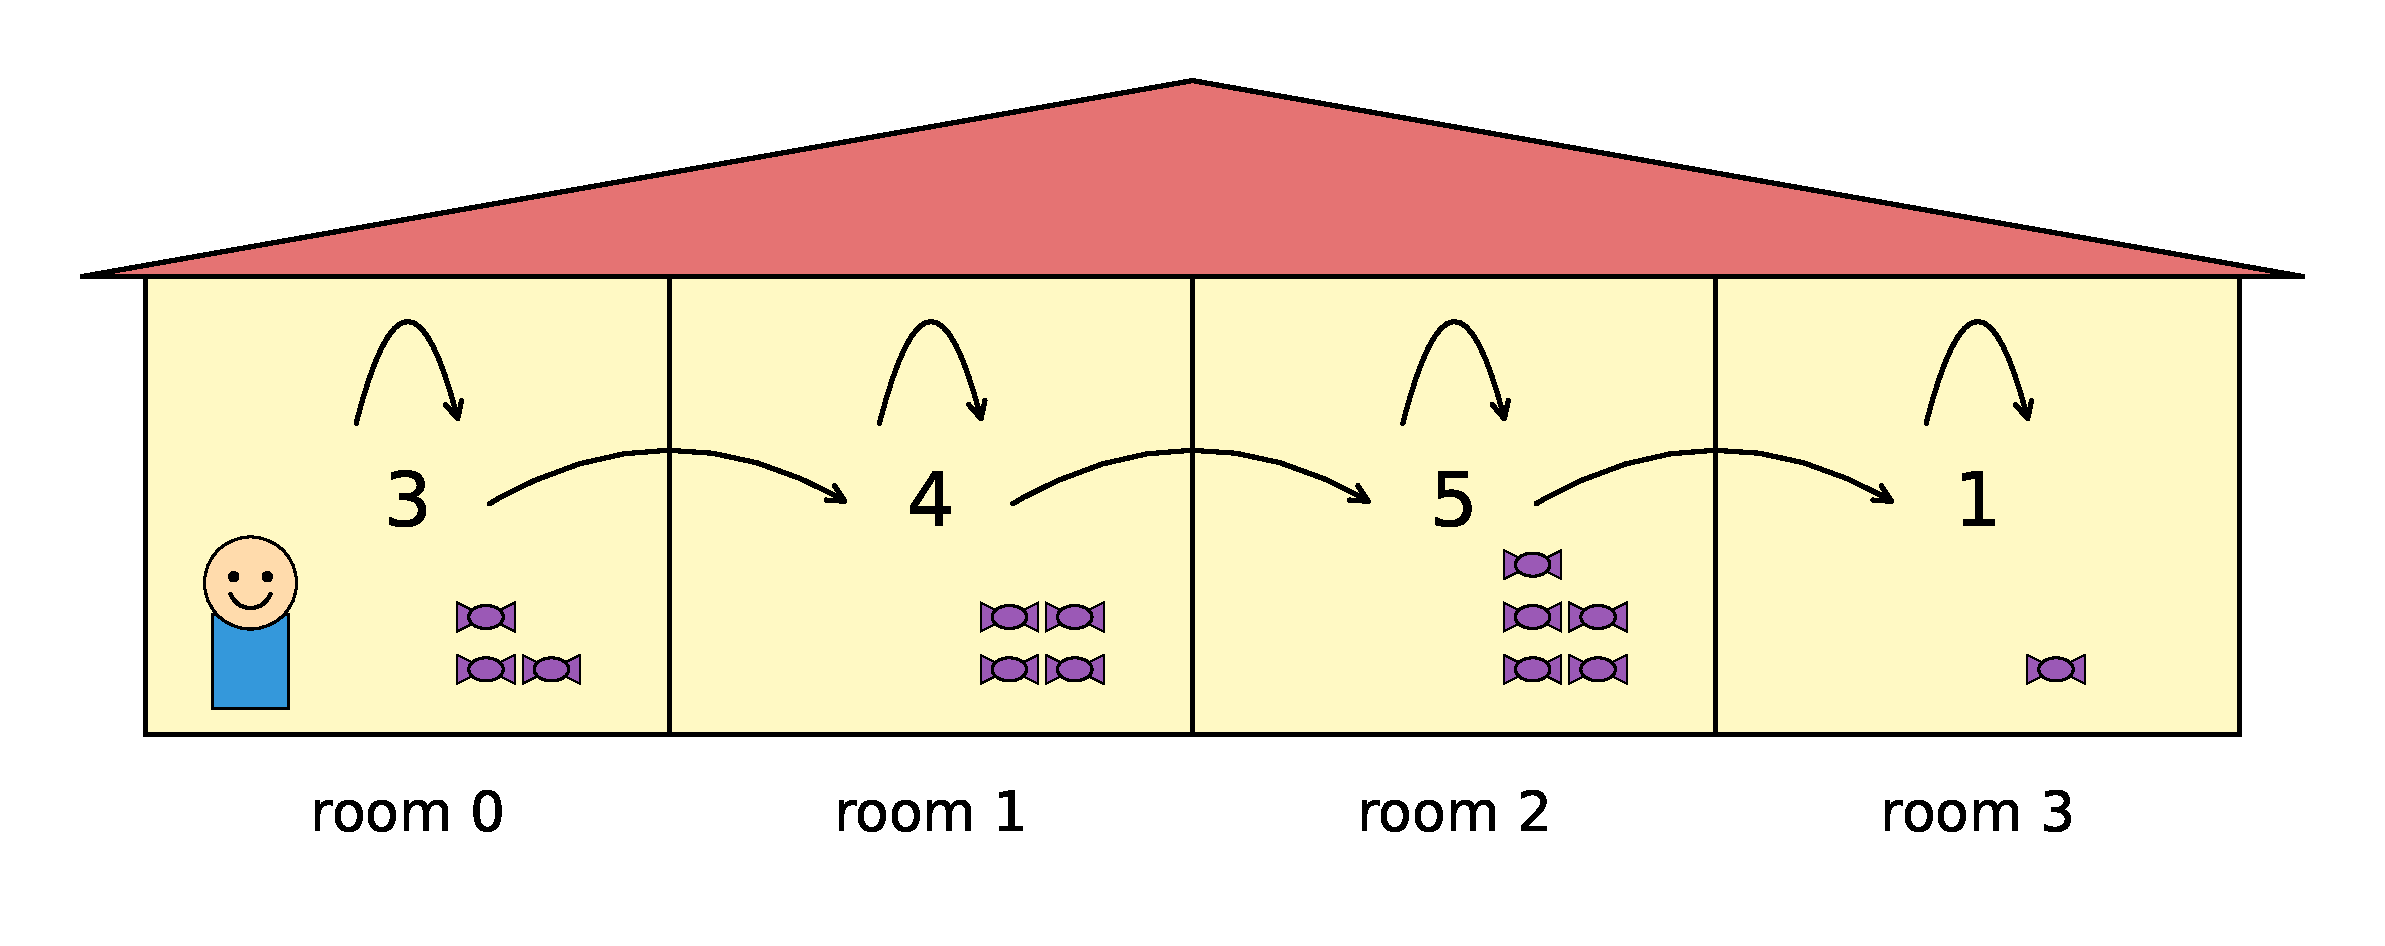
\includegraphics[width=0.8\textwidth]{candy_collection_2.pdf}
\end{center}

\newpage

\item[Problem 10] What is the optimal behavior in the following case with $r = \frac{1}{2}$?\\
How about $r = \frac{3}{4}$ (You care a lot about the future)?

\begin{center}
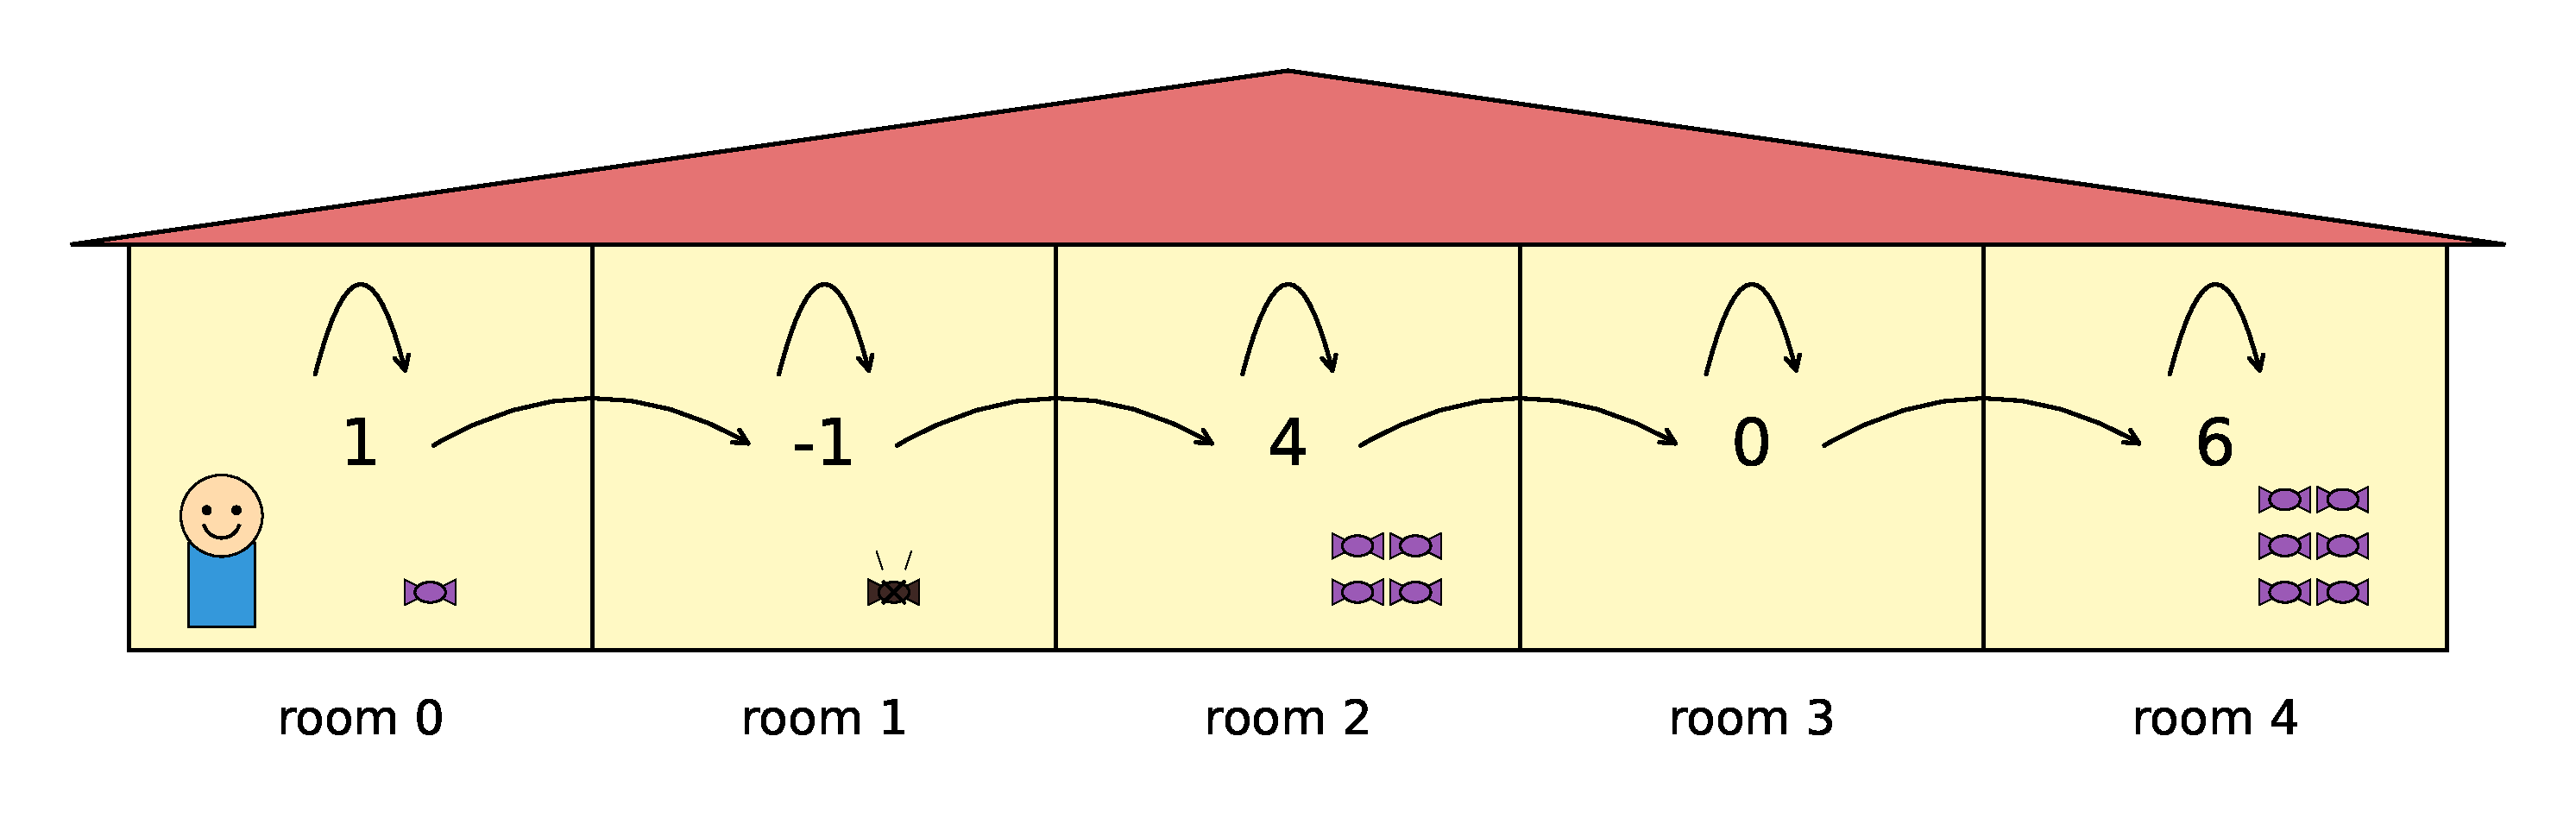
\includegraphics[width=\textwidth]{candy_collection_3.pdf}
\end{center}

 \end{description}

\newpage
\clearpage

\section{Edit distance}

The (minimum) edit distance is the number of (i) insertions of a single letter, (ii) deletions of a single letter, or (iii) substitutions of a single letter to turn one word to another?

\bigskip

Q: What is the edit distance between
\begin{enumerate}
\item ``CART'' and ``CAR''?
% = 1
\item ``FROM'' and ``FORM''?
% $\to$ A: 2
\item ``NEAR'' and ``EARN''?
% $\to$ A: 2
\item ``SUNDAY'' and ``SATURDAY''
% $\to$ (A: 3) but nontrivial.
\end{enumerate}

$d(i, j) =$ minimal number of edits to turn the first $i$ letters of ``NEAR'' into the first $j$ letters of ``EARN''.
\begin{itemize}
\item $d(1, 1) = \text{``N'' } \to \text{ ``E'' } = 1$,
\item $d(1, 2) = \text{``N'' } \to \text{ ``EA'' } = 2$.
\end{itemize}

Bellman equation:
\begin{equation}
d(i, j) = \begin{cases}
1 + \min \left\{ d(i-1, j), d(i, j-1), d(i-1, j-1) \right\} & \text{ if } S(i) \neq T(j),\\
d(i-1, j-1) & \text{ if } S(i) = T(j).
\end{cases}
\end{equation}

We do it via a \underline{$d$-table}.

\begin{description}

\item [Problem 11]  \ 

\begin{enumerate}
\item What is the edit distance from ``NEAR'' to ``EARN''? We know the answer more intuitively, but check it by creating the $d$-table.
\item From ``LEAST'' to ``STEAL''?
\item From ``CAMELY'' to ``BALLET''?
\item From ``SELLER'' to ``REELLS''?
\item From ``SUNDAY'' to ``SATURDAY''?
\end{enumerate}

\end{description}

\end{document}
